\subsubsection*{Maximum delay of an infix proof}
The problem with this infix proof construction is that in order to confirm a
transaction in a block of interest $b$ the prover has to provide an inclusion
proof for that block of interest using the Merkle Tree Root of a more recent
honestly generated block included in the infix proof. Obviously, there is a case
that there may be a number of consecutive adversarially generated blocks in the
chain   consisting the prefix of the chain. Thus, no inclusion proof can be provided
for any of these blocks until an honestly generated block is added in the chain and,
consequently in the infix proof.

We need to estimate an upper bound for the number of rounds a client has to
wait until the block of interest is buried under sufficient number of blocks
so that he can obtain the infix proof needed with high probability.

Consider $n_b$ is the upper bound on the consecutive rounds when the adversary could
possibly append blocks to the chain, without any honestly generated blocks in
between. The adversary mines either by following the selfish mining strategy or
not. The state of the chain we examine looks like in Figure \ref{fig:infix_delay}.

\begin{figure}[h!]
	\begin{center}
		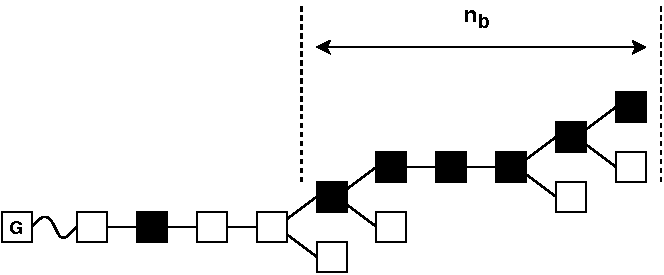
\includegraphics[width=0.8\columnwidth]{figures/infix_delay.pdf}
	\end{center}
	\caption{ \textbf{$n_b$} implies the number of consecutive
	 adversarially generated blocks in the chain.Wavy lines imply one or more blocks. Blocks generated by the
	 adversary are colored black.}
	\label{fig:infix_delay}
\end{figure}

Let $p_H$ the probability that a block is generated by an honest party during a round.
Then considering that collisions in RO model is a negligible event we have
$p_H = (n-t)qp$. Let $p_A$ be the probability that a block is generated by the
adversary during a round, then $p_A = tqp$. Consider $N_{bA}$ the random variable
for the number of consecutive blocks generated by the adversary in a total of $r$
rounds. Also let $N_{bH}$ the random variable for the number of blocks generated by
honest parties in total of $r$ rounds. 
Then we have that $N_{bA}$, $N_{bH}$ follow the Binomial Distribution with
probability $p_A$, $p_H$ respectively.

Because we require consecutive successful rounds for the adversary, we have:
\begin{equation}
	Pr[N_{bA} = n_b] = (r-n_b - 1) p_A^{n_b}(1-p_A)^{r-n_b}
\end{equation}

while for the honest players we have 
\begin{equation}
	Pr[N_{bH} \leq n_b] = \sum_{i=0}^{n_b} \binom nk p_H^{i}(1-p_H)^{r-i}
\end{equation}

If $N_b$ is the random variable denoting the number of consecutive rounds that
adversarially generated blocks are appended to the chain, we have:

\begin{equation}
	Pr[N_b = n_b] = Pr[N_{bA} = n_b] \cdot Pr[N_{bH} \leq n_b]
\end{equation}

since the two events are independent.